Windows System Restore is een functie van Microsoft om je systeem te helpen beschermen tegen het corrupt raken van systeemsettings. Het wordt voornamelijk gebruikt voor het terugdraaien van recente wijzigingen veroorzaakt door software installaties, driver installaties of wijzgingen in systeemsettings. Het terug gaan naar een vorig moment (restore point) herstelt het systeem zonder dat je documenten worden terug gezet. Je raakt dus geen persoonlijke data kwijt.

System Restore werkt door Restore Points te maken, dat zijn een soort snapshots van de systeemconfiguratie op een specifiek moment. De restore points kunnen automatisch gemaakt worden, maar je kan ze ook handmatig maken, bijvoorbeeld vlak voor een installatie of update van een stuk software. Een restore naar een vorig restore point zet system files, registry settings en ge\"installeerd programma's terug naar de status waarin ze waren toen het restore point werd gemaakt.

Windows System Restore monitort bestanden met een bepaalde extensie. De lijst met extensies die gemonitord worden kan je vinden op \url{https://learn.microsoft.com/en-us/windows/win32/sr/monitored-file-extensions}.

Standaard staat het maken van Restore Points uit in Windows. We zullen het dus eerst aan moeten zetten. Om dat te doen gaan we naar Advanced System Settings. In de tab System Protection kunnen we door op \textquote{Configuration} te klikken system protection aan zetten.

\begin{minipage}[t]{\linewidth}
\raggedright
\adjustbox{valign=t}{%
   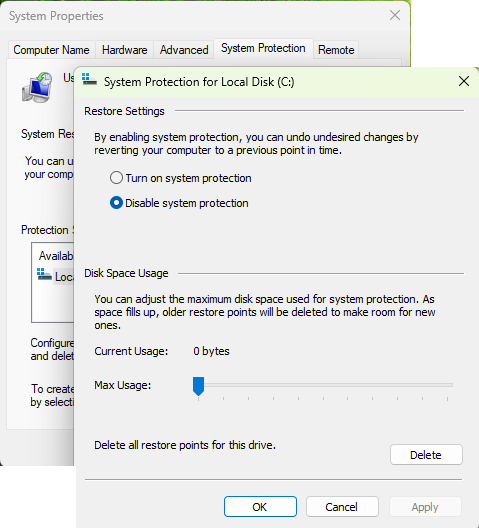
\includegraphics[width=0.75\linewidth]{system_protection-on.png}%
}
\end{minipage}

Selecteer \textquote{Turn on system protection} en je kan aangeven wat de maximale hoeveelheid ruimte is die restore points in mogen nemen.

In het hoofdpanel kan je nadat we system protection aan hebben gezet bij \textquote{Create...} een eerste restore point maken.



